\chapter{Deep Learning Techniques}
\label{chap:MLTechniques}
%%%%%%%%%%%%%%%%%%%%%%%%%%%%%%%%%%%%%%%%%%%%%%%%%%%%%%%%%%%%%%%
% Outline 
% Introduce Machine Learning, and why traiditonal FCN is not good enough
% 1. Convolutional Neural Networks
% 1.1 Example architecture and sucess in vision tasks
% 1.2 1D CNN implemented on DESI spectra
% 1.3 2D CNN implemented on DESI spectra (Eddies Research)
% 2. Transformers 
% 2.1 Example architecture and sucess in NLP tasks + Vision Tasks --> Connection 
%      to DESI
% 2.2 Multi-Head Attention and Self-Attention for spectral classification
% 2.3 Possilbility of NOT having to k-correct for redshift because of this attention
% 2.4 Adjected ViT architecture for DESI

%%%%%%%%%%%%%%%%%%%%%%%%%%%%%%%%%%%%%%%%%%%%%%%%%%%%%%%%%%%%%%%
To aid in the classification of supernovae, deep learning techniques can provide 
flexibility and scalability that have been previously unattainable by manual 
methods. The simplest form of machine learning algorithms are the feed-forward 
fully connected neural networks (FCNs). These networks apply a series of linear 
transformations to the input data, followed by a bias and a non-linear activation 
function. The output of the network is another vector tailored for whatever the 
purpose of the FCN is (i.e. for classification, is a vector of probabilities 
that the input data belongs to, see Appendix~\ref{app:FCN}). 

This architecture, while simplistic, is very powerful. \textcite{cybenko1989} showed that for any boolean 
function (i.e. 2 class classification), a FCN with a single hidden layer could 
approximate any function arbitrarily well; this is known as the universal approximation
theorem. The theorem is the basis for the success of FCNs in
many fields, but also the reason that FCNs are not the best choice for all problems.
The main issue with FCNs is that they are not invariant to translations, which is 
essential for many problems, such as image recognition, time series analysis, and 
natural language processing. Therefore, alternative options have been proposed. 

\section{Convolutional Neural Networks}\label{sec:CNN}
Convolutional neural networks (CNNs) were originally developed as a solution 
to positional differences in the input data \parencite{fukushima1979}. This architecture 
was shown to be effective in image recognition tasks by \textcite{lecun2004} and then popularized after the success of AlexNet in the 
ImageNet challenge \textcite{krizhevsky2012}. The networks have since been applied to
many other vision tasks and various fields, such as NLP and audio processing. 
CNNs are composed of a series of convolutional layers, usually followed by a 
pooling layer and a fully connected layer (Appendix~\ref{app:CNN}). The convolutional layers are composed of a series of convolutional filters, which are commonly referred to as feature maps.
The convolutional filters are applied across the entire input space giving the CNN its invariance to translations.

\subsection{CNNs on Spectroscopic Data}
\label{sec:CNNspectra}
CNNs are especially good at identifying patterns throughout their input space, stemming from their spacial invariance. Theoretically, this should translate to spectral classification quite well. In fact, CNNs have been applied 
to spectroscopic data in the past, even on the DESI dataset. 
\textcite{parks2018} used a CNN to detect strong emission lines in DESI spectra with 
great success. * Talk about 1D CNN currently running, and preprocessing used *

This work provides a baseline for the use of CNNs on supernovae classification, 
but leaves more to be desired. Therefore, an alternate architecture was proposed 
by * Cite Eddies work * which augments the preprocessing of the spectra with 
a conversion to a 2D image. This 2D image was then fed to a more traditional vision 
CNN architecture (Appendix~\ref{app:CNN}). 
\begin{figure}[h]
    \centering
    \subfloat[\centering~ROC curve]{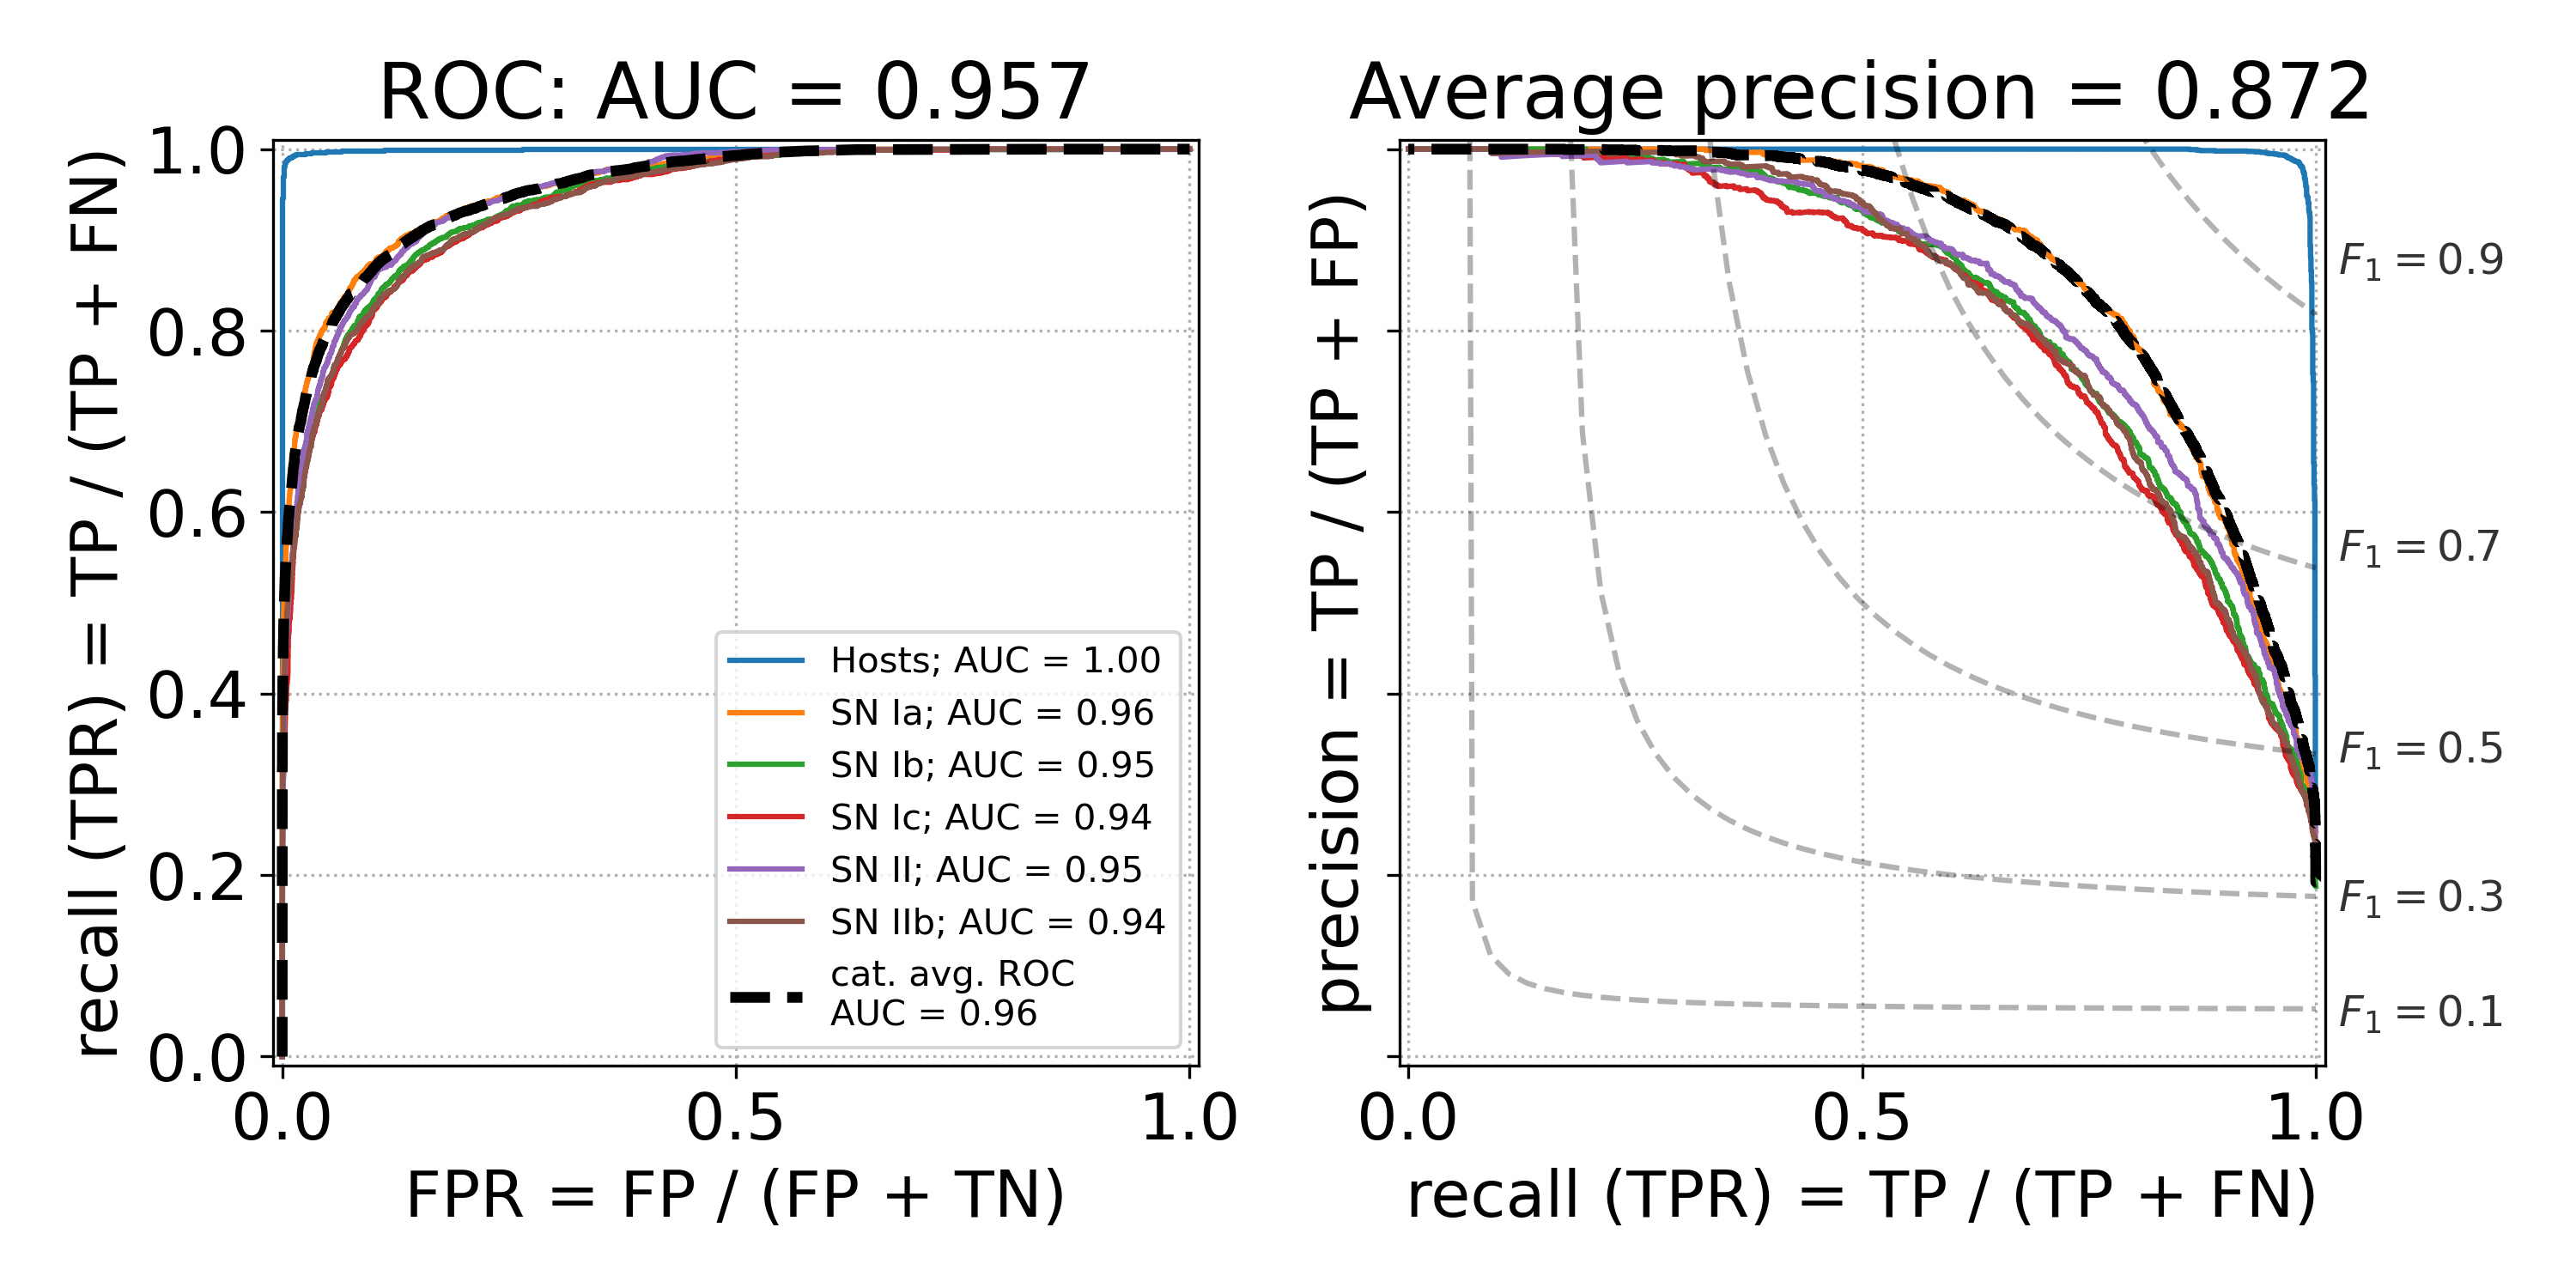
\includegraphics[width=5cm]{figures/cnn/cnn_rocfull.png}}
    \qquad
    \subfloat[\centering~Confusion Matrix]{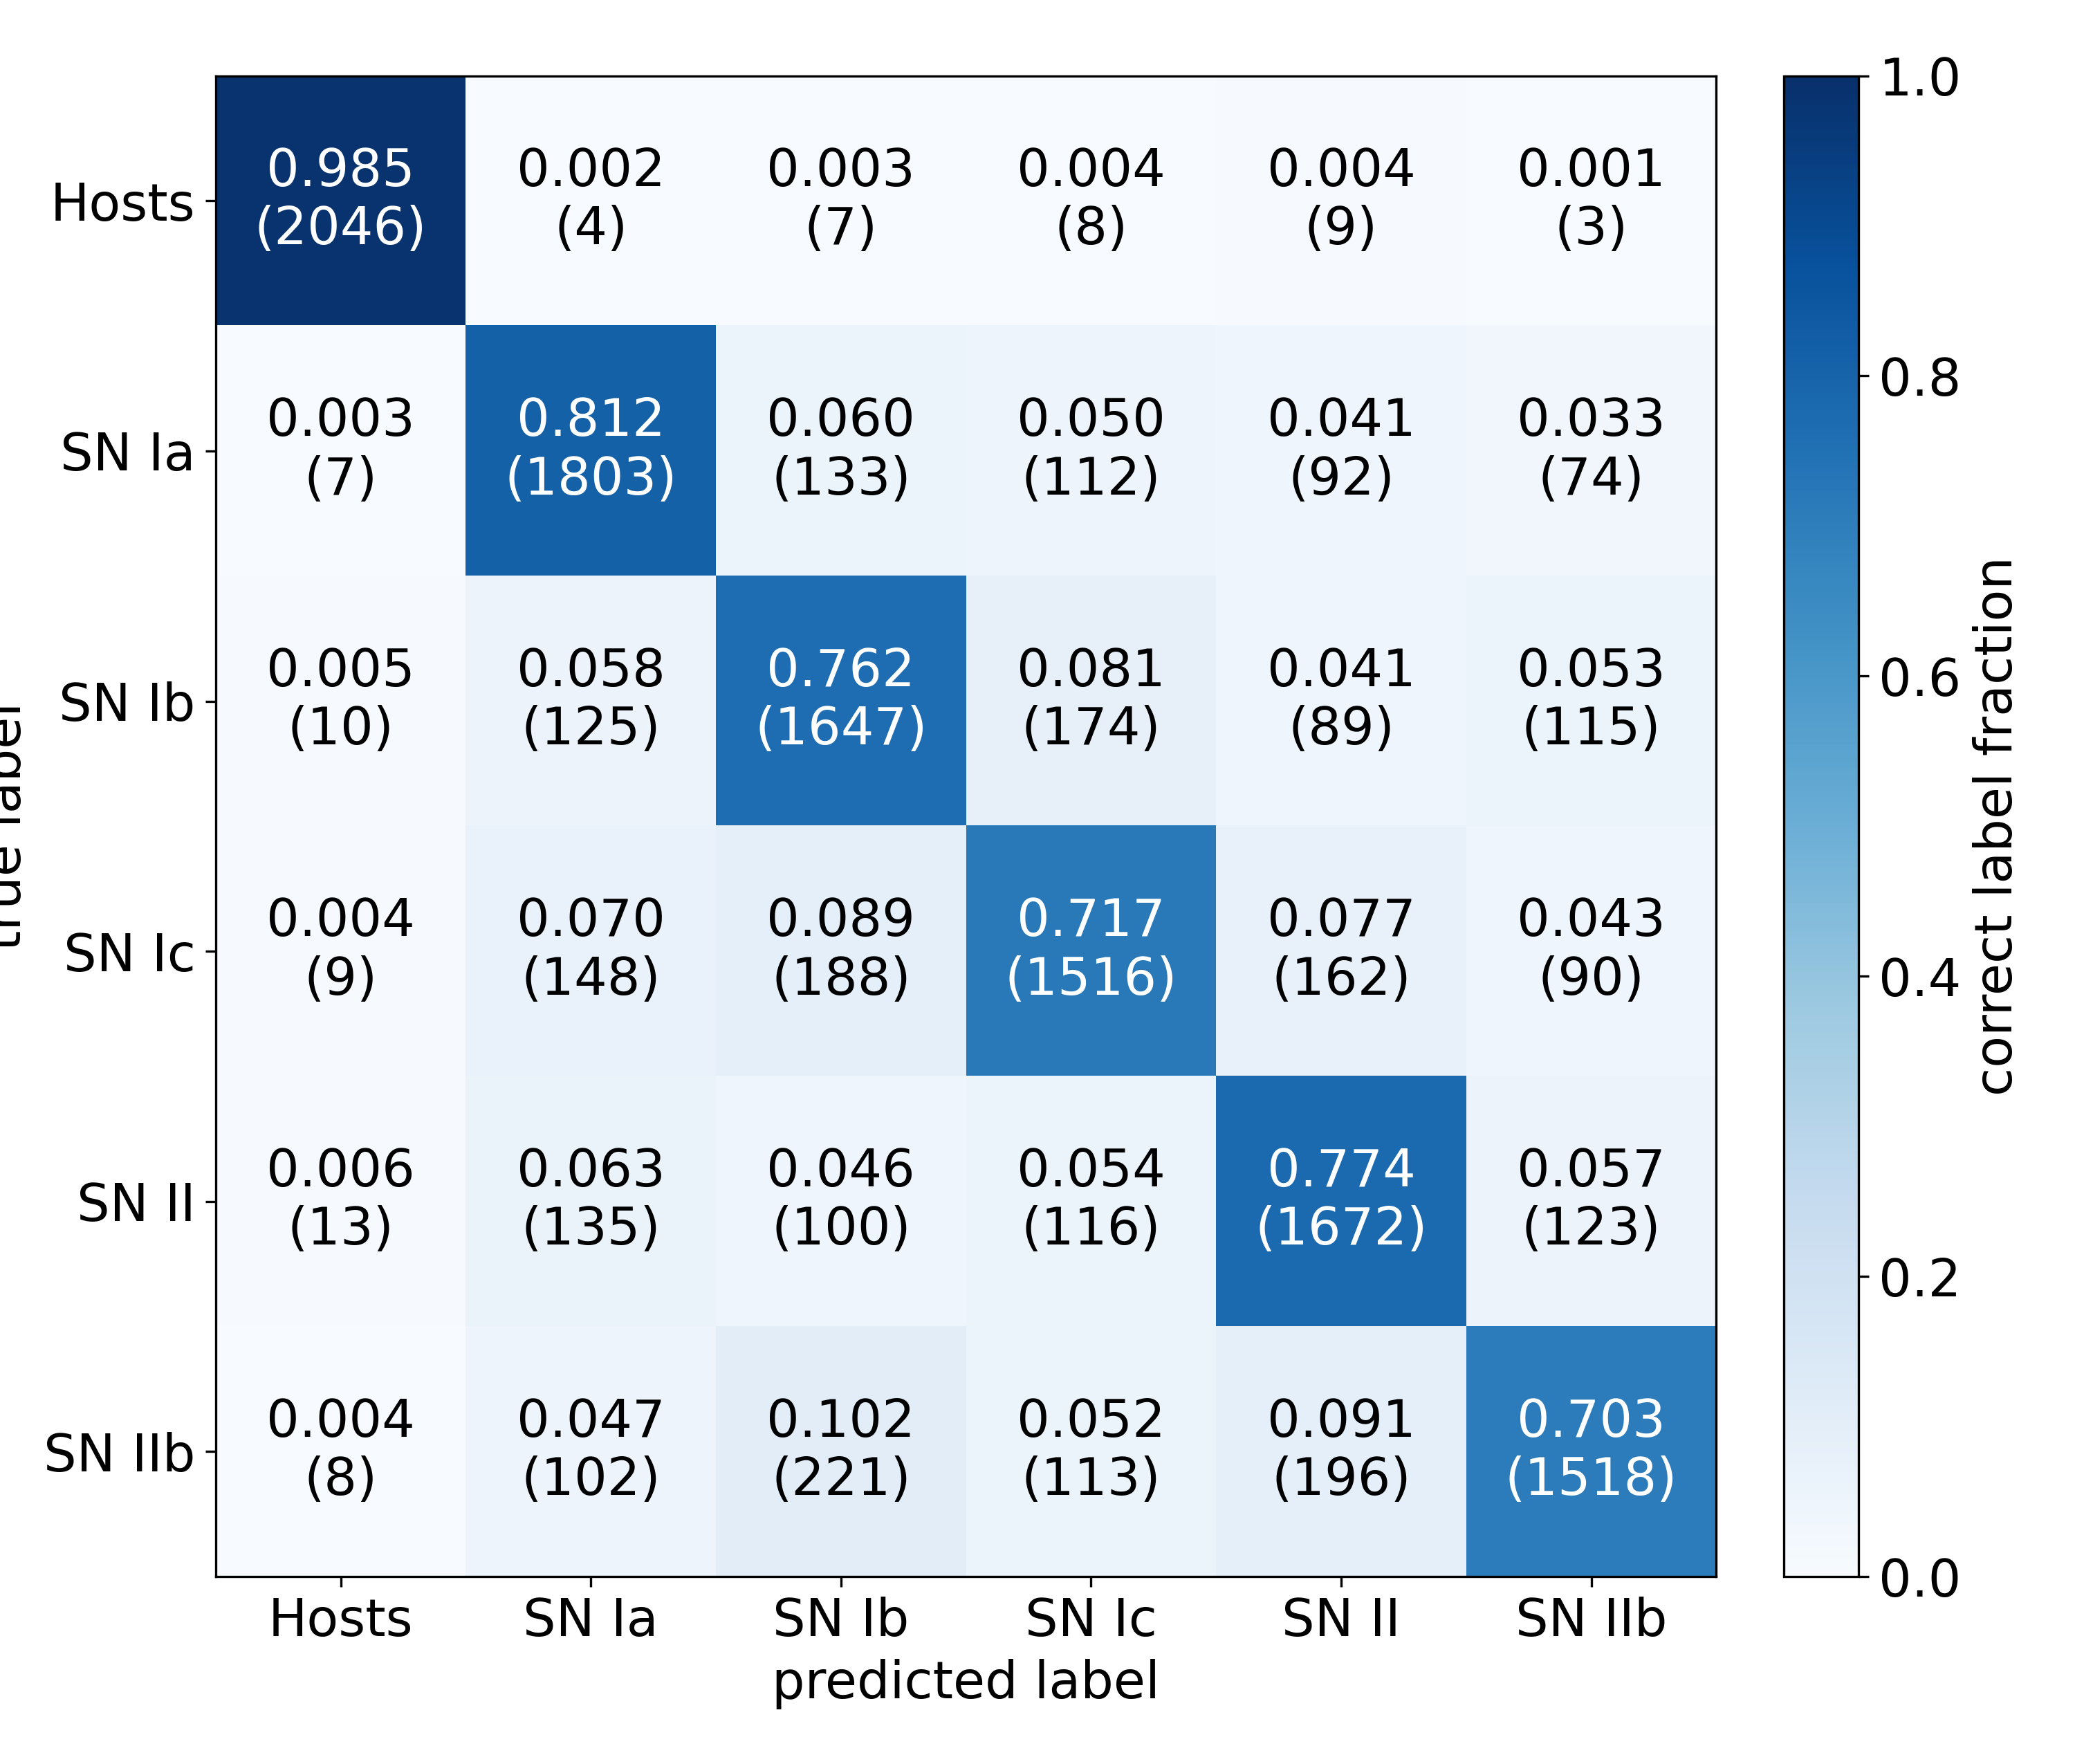
\includegraphics[width=5cm]{figures/cnn/cnn_cmfull.png}}
    \caption{CNN Diagnostics\label{fig:cnn_qual}}
\end{figure}
This architecture was shown to train quickly (less than 1 hour on a single GPU), 
but was not able to achieve astonishingly high accuracy. Figure~\ref{fig:cnn_qual}
shows the ROC curve and confusion matrix for the CNN trained on synthetic spectra. 
\begin{figure}[h]
    \centering
    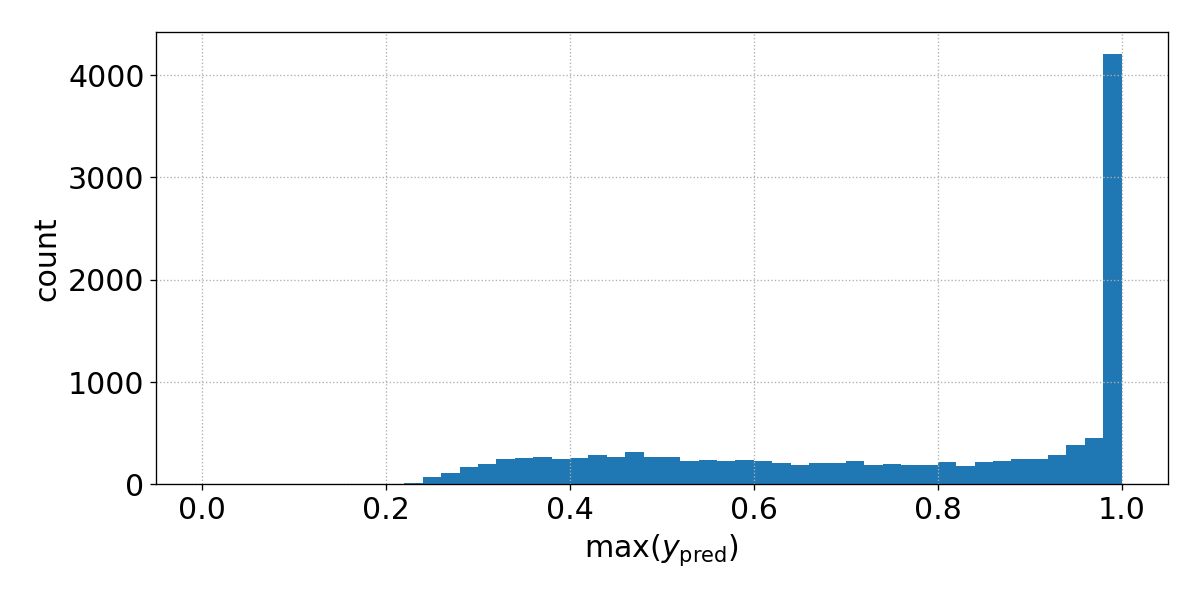
\includegraphics[width=0.5\textwidth]{figures/cnn/cnn_max_ypred.png}
    \caption{Max value of the output vector for the CNN.\label{fig:cnn_max}}
\end{figure}

The maximum value of the output vector was used to determine the predicted class,
which may not be the best choice for this problem. Figure~\ref{fig:cnn_max} shows
the distribution of the maximum value found. As shown, there are approximately 
20 thousand spectra that are classified very confidently, but there are many
more that are not.
\begin{figure}[h]
    \centering
    \subfloat[\centering~ROC curve]{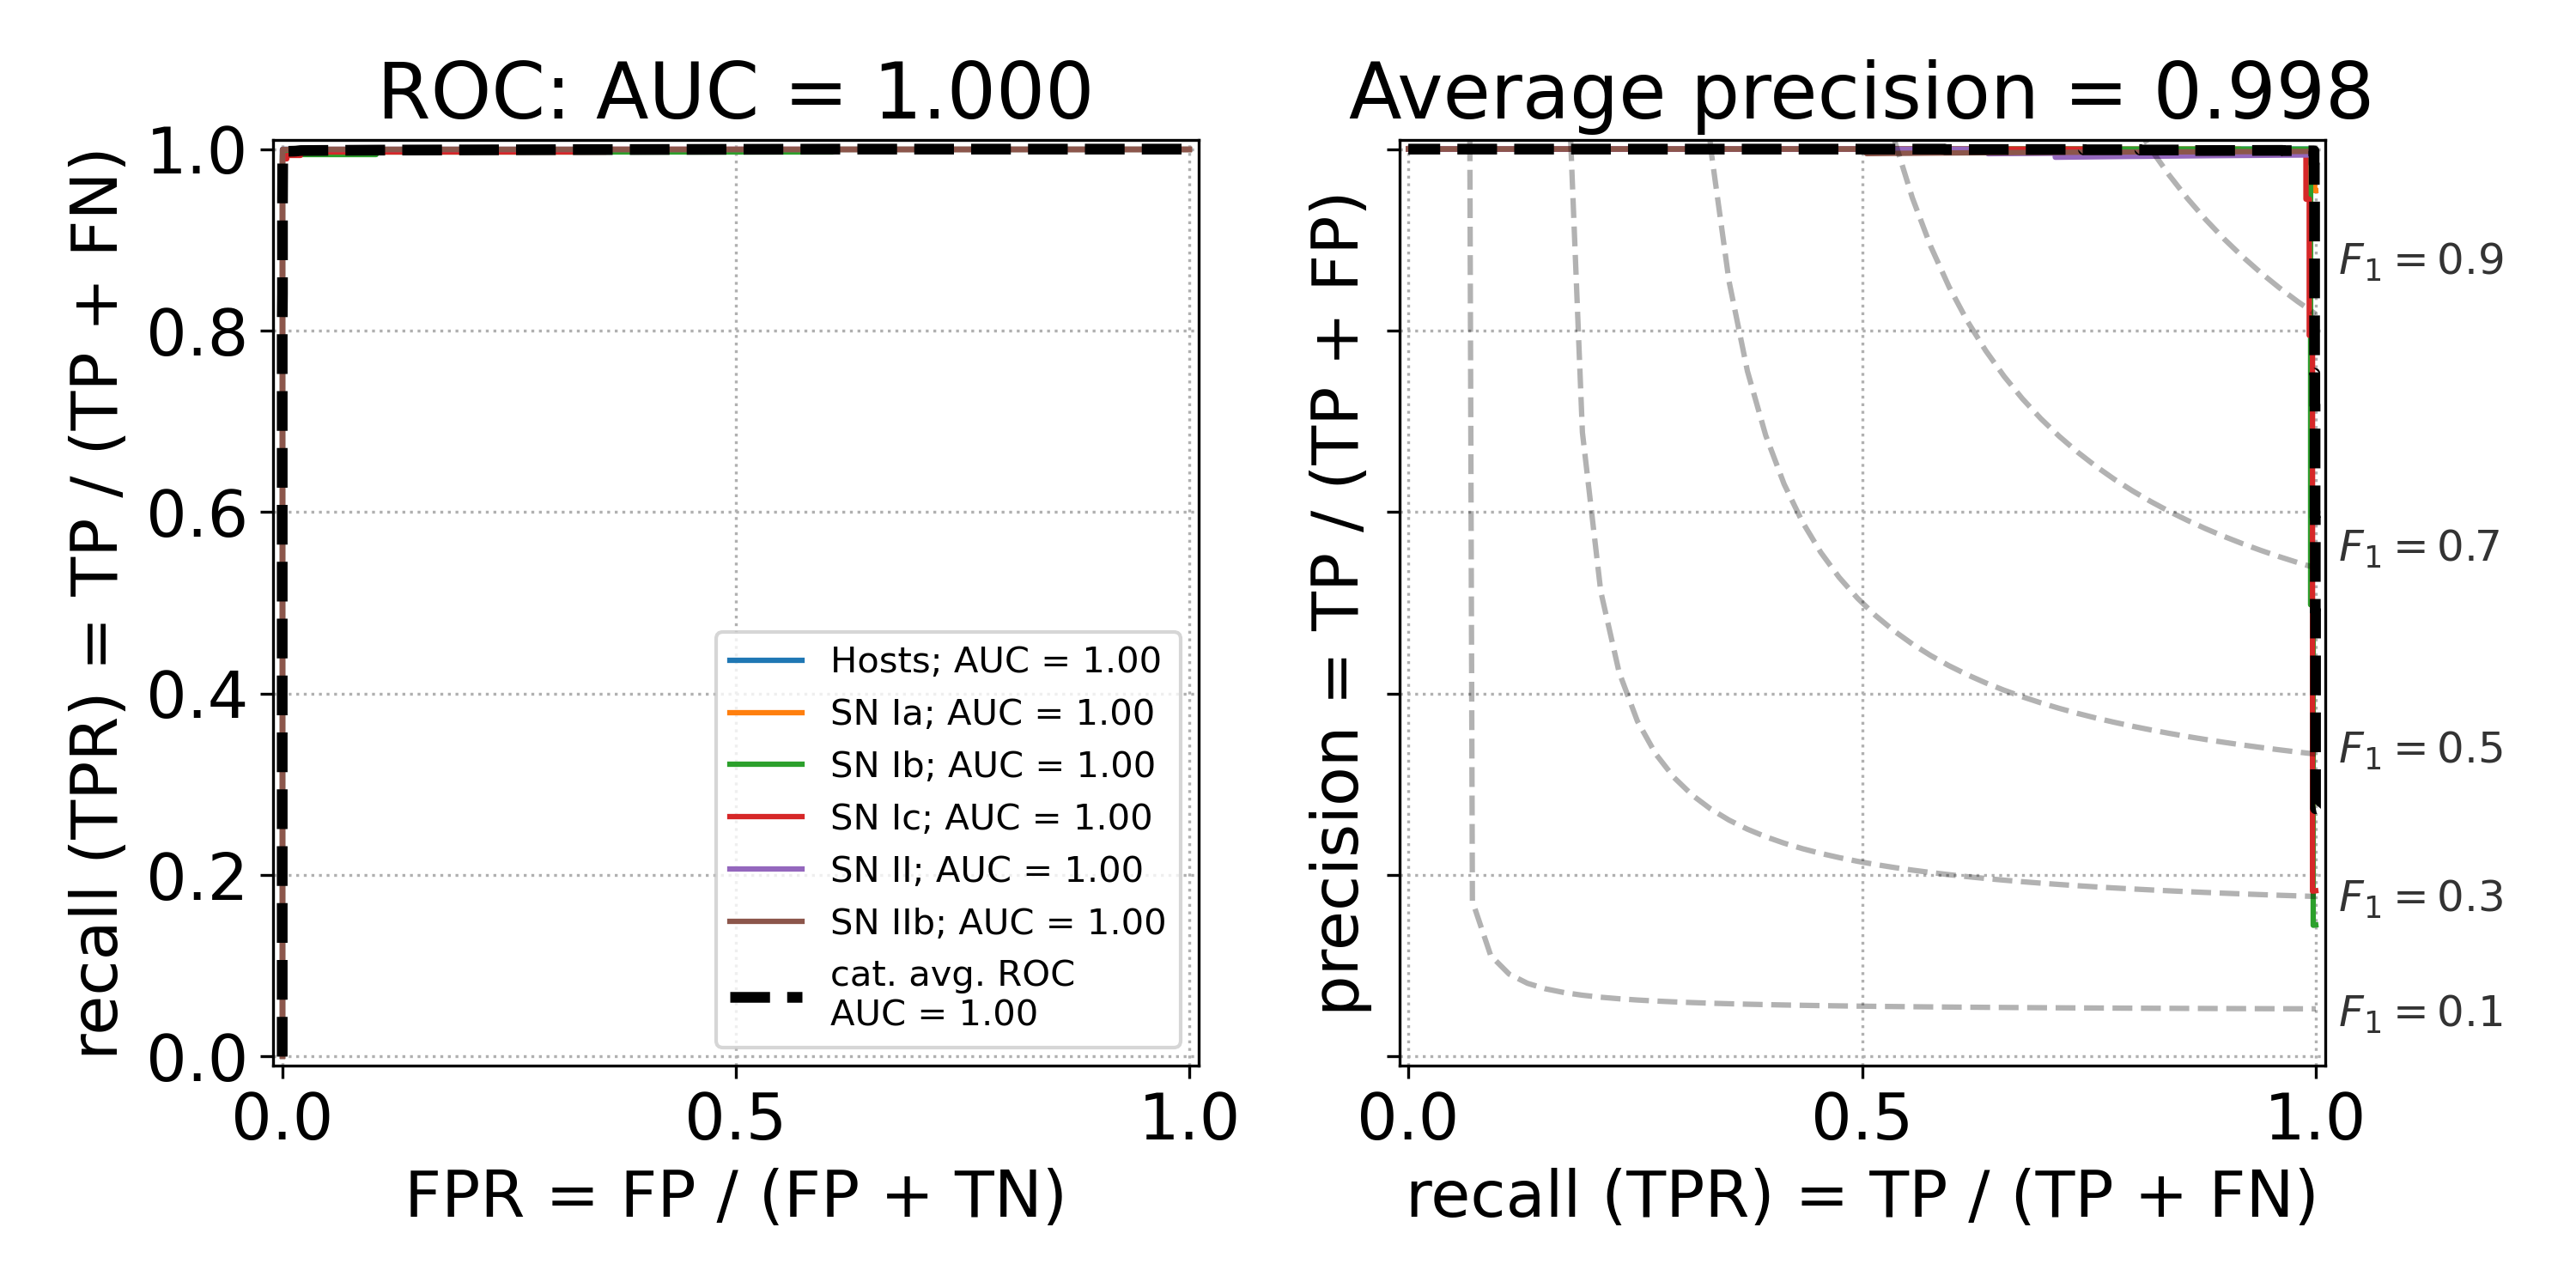
\includegraphics[width=5cm]{figures/cnn/cnn_roc99.png}}
    \qquad
    \subfloat[\centering~Confusion Matrix]{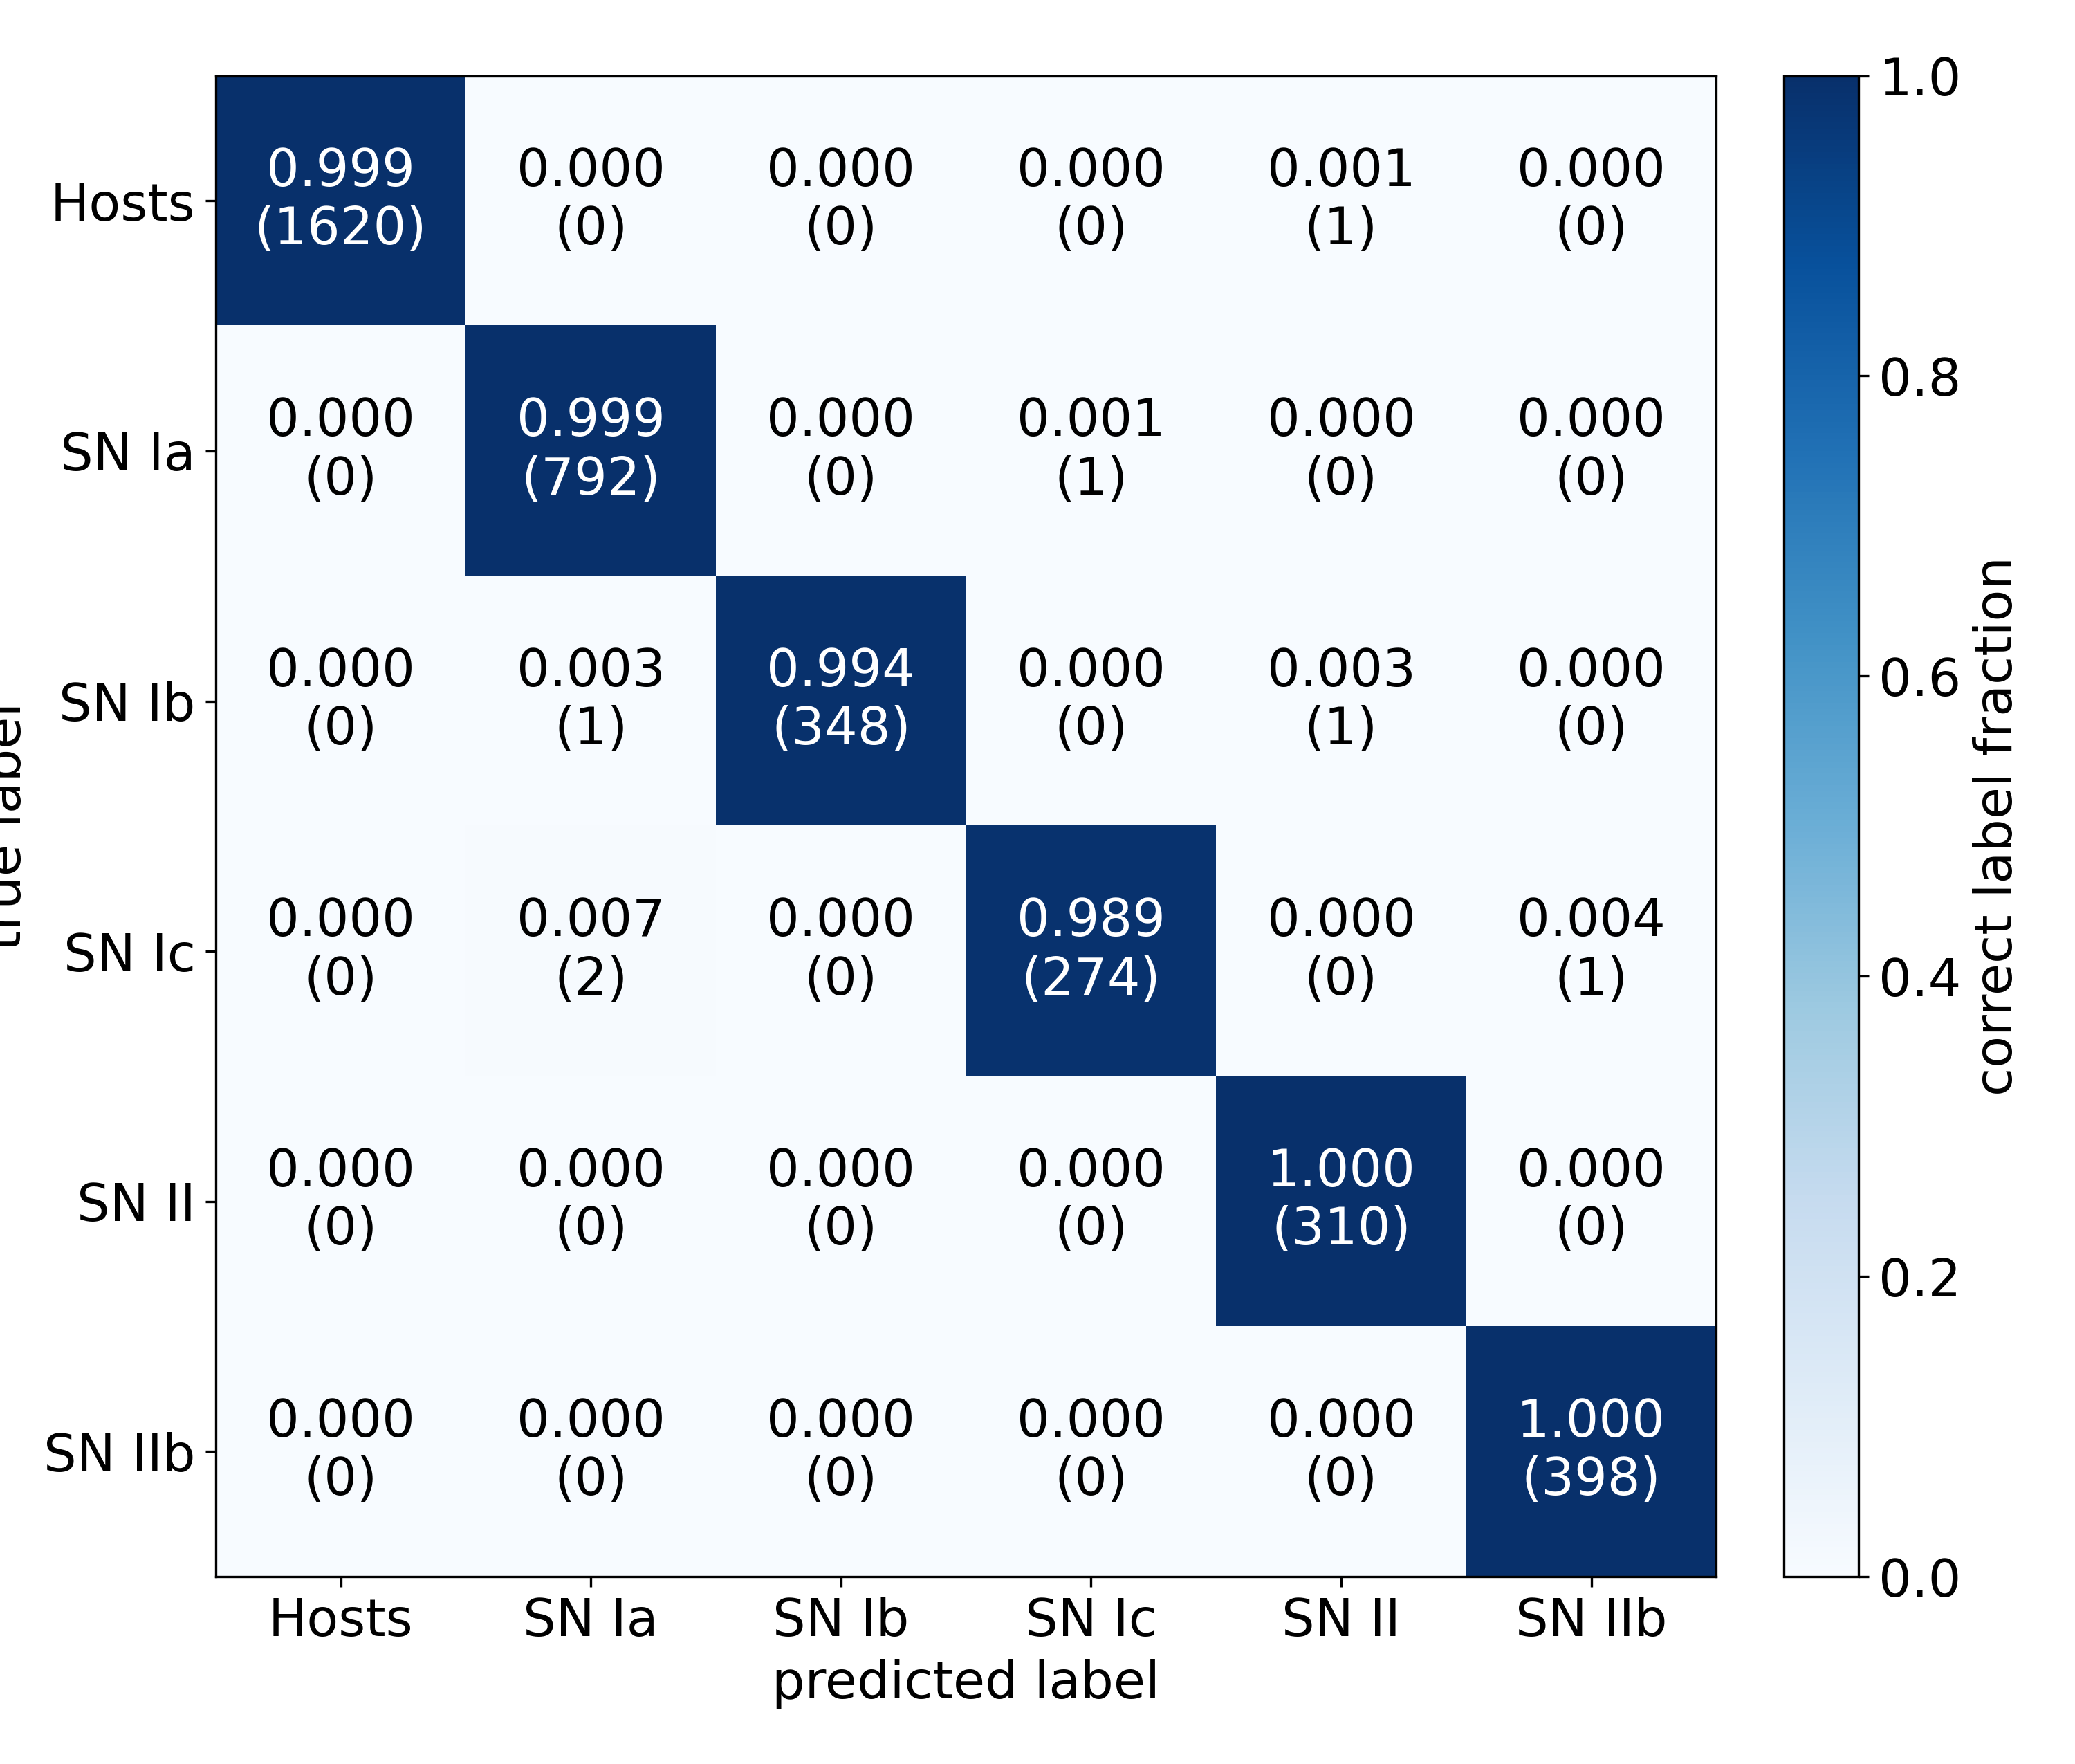
\includegraphics[width=5cm]{figures/cnn/cnn_cm99.png}}
    \caption{CNN Diagnostics\label{fig:cnn_qual2}}
\end{figure}

Taking a look at the diagnostics again, but only for highly confident classifications,
a much better ROC curve and confusion matrix is produced (Figure~\ref{fig:cnn_qual2}). 
Therefore, it is clear that the CNN, when confident in its classification, produces 
accurate results. This cut, however, is not ideal, removing *insert percent*\% of the 
data. 

The next step in training would be to either increase the confidence of the CNN, 
or to move to a different architecture, with the hopes of increasing not only 
the overall accuracy of the networks, but also the number of confident classifications.
% This begs the question, which is more important? The ability to classify a lot of 
% spectra with low confidence, or a few spectra with high confidence? Even if a 
% cut was made on the confidence of the classification, would the optimal solution
% yield better results under the same conditions? 

\section{Introduction of Transformers}\label{sec:transformers}
% Advantage of transformers in this field
Transformers are a relatively new architecture, first introduced in 2017 by \textcite{vaswani2017}
for natural language processing (NLP) tasks. The original architecture consists of 
an encoder-decoder system. The encoder accepts a series of tokens, and via a series 
of self-attention layers and feed-forward layers, produces a series of vectors
representing the input data. The decoder then takes the output of the encoder, and
produces a series of tokens, one for each input token. 

Once transformers were shown to have remarkable success in NLP tasks, they were 
quickly adapted to other fields, such as vision. \textcite{dosovitskiy2020} developed 
a vision transformer (ViT) architecture that differed from the original transformer 
encoder by replacing the tokenized input with a more involved preprocessing step. In short, 
the input image is broken into a series of patches, which are then flattened into
a vector. These vectors, along with positional encodings, are then fed into the
transformer architecture. For classification tasks, the first input token is 
replaced with a class token. After passing through the transformer, the class token 
is then run through a fully connected layer to produce the final probabilities. 

\subsection{ViT on Spectroscopic Data}\label{sec:ViT}
Previous implementations of transformers have been shown to have characteristics 
beneficial to the classification of spectral data. A transformer's 
ability to learn contextual information is essential in spectral classification. 
A broad absorption line, for example, may be indicative of a Type Ia supernova 
if in one part of the spectrum, but may be indicative of a Type II supernova if
in another part of the spectrum. This contextual information is not easily learned 
by a CNN, as the convolutional layers are not able to learn the importance of
certain parts of the input space. Attention can also play a role in identifying 
the purpose of features that are not in a standard location. For example, a 
non-k corrected spectrum might have a continuum pattern at different locations 
in the spectrum, but the overall shape would be similar. This change in sizing 
would be difficult to learn with fixed filters in a CNN, but would be identified 
based on their positional importance by a transformer. In addition to this, ViTs 
have been shown to outperform CNNs on vision tasks, which shows they are capable 
of focusing on learned features. 


* Include caveat about the fact that ViTs take longer to train than CNNs *

